\chapter{Introduction}
\label{chap:introduction}

\drop{T}{oday} each of Facebook, Twitter and Linkedin~\cite{facebook, twitter, linkedin}
ingest more than 12M events per second. Another important automated data source
is Internet of Things~\cite{iot} that is bringing even larger volumes of data
that are predicted to double every year. The plunging cost of data storage,
accelerated by cloud computing, is enabling many companies to collect and store
huge amounts of data. The analysis and exploration of these data sets can change
ad-hoc business decisions to data-driven ones, with higher probability of being
successful.

\noindent
There are many scenarios where data analysis can play a big role:

Web companies do \textit{behavioral analytics} so they can study how their customers use
their platforms. This enables actions like \textit{session targeting}. This consists of
special offers depending on what the customer is doing while using the service,
increasing the chances of successful commercial transactions.

Another related action could be \textit{campaign optimization}. One of the biggest
business in internet is advertising. Companies that are able to generate the best
return for the advertisers are the ones that will overcome the competition.

New technological architectures, like microservices-based, provide solutions to
problems that before were almost impossible to solve, such as scalability. There is
a cost associated with this architecture: monitoring these services. Companies
like Netflix have thousands of services running~\cite{netflix}, and some of those
services can produce over 40.000 metrics per second. Analyzing metrics data is
key to being able to detect anomalies, degradation in services and without doubt
the only way to run large distributed systems.

But it does not end here, as there are many more examples where data analytics
is fundamental. Scientific experiments, i.e. CERN (generates terabytes of data, per
experiment)~\cite{cern}, security, and many more that are arising over time.

\begin{figure}[!h]
\begin{center}
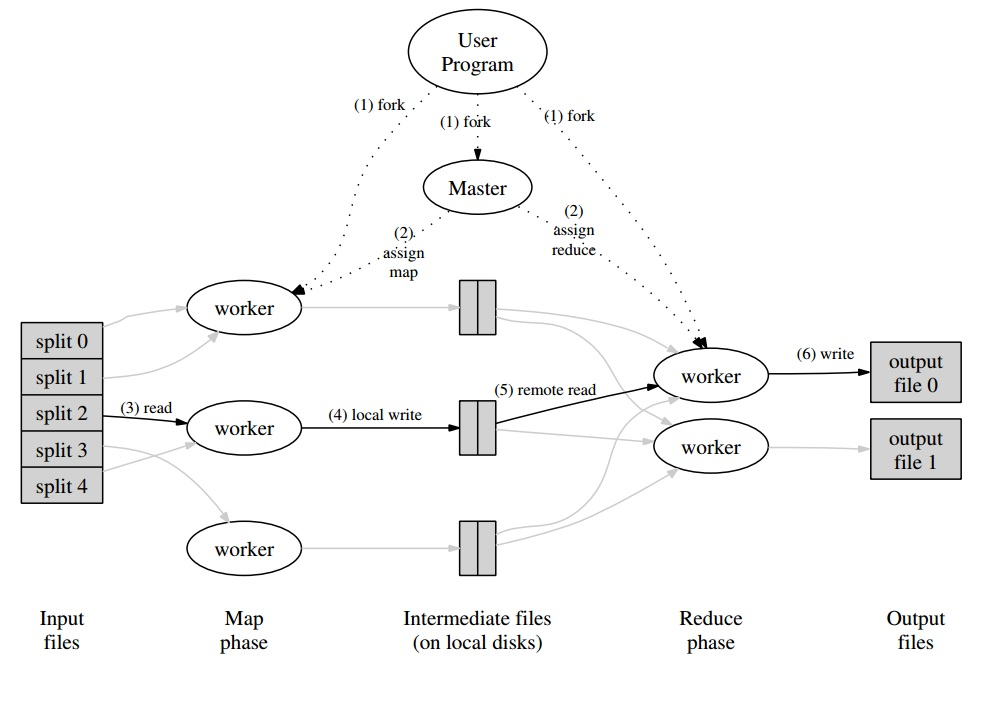
\includegraphics[width=1\textwidth]{mapreduce.jpg}
\caption{Map-Reduce architecture~\cite{mapreduce}}
\label{fig:mapreduce}
\end{center}
\end{figure}

Traditional DBMS cannot cope with the scale and heterogeneity of the data sets
cited previously. Over time, models like MapReduce~\cite{mapreduce}
Figure~\ref{fig:mapreduce}, Spark~\cite{spark} and Storm appeared. Those
architectural models facilitated the parallelization of data analysis processes
at scale, running on commodity hardware. These systems are classified as batch
processing, meaning that all input should be collected into a batch before
processing it.

MapReduce and batch processing paradigms have been quite successful over the
years on large data-sets scenarios. But new needs are arising
and data analysts are becoming more demanding with their requirements. Batch
systems are designed to run with bounded data, imposing big latencies. In some
situations it is not feasible to wait hours to get back results from analytics.
One example could be monitoring microservices architectures where anomalies must
be investigated and fixed as soon as possible to avoid service disruptions.

To avoid latencies imposed by batch systems, hybrid systems were designed. One
paradigmatic example is Lambda Architecture~\cite{lambda}. It consists of
two data processing systems running in parallel. One of the systems, known as
streaming system, will provide approximate results in nearly real time. To
obtain more precise results, a classic batch systems run over the same data-set.
Soon, these systems showed many problems. Running two processing pipelines in
parallel is translated into many operational issues as well as more costs~\cite{kappa}.

In general, batch processing systems don't perform well on stream data-sets.
Stream data-sets, as defined in~\cite{streamissues}, can be characterized as follows:
%
\textit{
\begin{itemize}
\item The data elements in the stream arrive online.
\item The system has no control over the order in which data elements arrive to
  be processed, either within a data stream or across data streams.
\item Data streams are potentially unbounded in size.
\item Once an element from a data stream has been processed it is discarded or
  archived — it cannot be retrieved easily unless it is explicitly stored in
  memory, which typically is small relative to the size of the data streams
\end{itemize}
}

It is clear that batch systems were one of the enablers of big processing pipelines,
but new data processing platforms are needed. In particular, data processing platforms
that are able to deal with stream data.

To overcome the limitations imposed by batch systems on streaming data, a few
alternatives appeared. Google developed MillWheel~\cite{millwheel} and Google
DataFlow~\cite{dataflow}. Those systems were designed with the previously presented
problems in mind. The main differentiator was how unordered data was treated. To
facilitate working with unordered events, the next concepts were introduced~\cite{dataflow}:
\textit{
  \begin{itemize}
  \item Windowing: slicing data into finite chunks for processing.
  \item Triggering: stimulating the output of a specific window at a grouping operation.
  \end{itemize}
}

This project will be focused on developing a data processing system using the
same principles that Google Dataflow and MillWheel are based on.

During the next chapters a description of the specific objectives of this
project, an exposition of the state of the art and the methodology used to
develop this project will be presented. Once these topics are introduced, a
detailed characterization of Alcaudon architecture is explained as well as the
accomplished results.

% Local Variables:
% ispell-local-dictionary: "american"
% End:
